% !TeX encoding = windows-1251
\documentclass[a4paper,12pt]{article}

\usepackage{newlistok}
\usepackage{tikz}

\УвеличитьШирину{1cm}
\УвеличитьВысоту{2.5cm}
\renewcommand{\spacer}{\vfil}

\Заголовок{Отображения}
\НомерЛистка{5}
\ДатаЛистка{10.2012}

\begin{document}


\СоздатьЗаголовок

\опр
Правило $f$, сопоставляющее каждому элементу $x$
множества $X$ некоторый элемент $y$ множества $Y$, называется \выд отображением из множества $X$ в множество $Y$. \\
Обозначения: $f\colon X \to Y$; $f(x)= y$; $x\stackrel{f}{\mapsto} y$.

\копр

%1. $X$ --- множество учеников, присутствующих на уроке в 14 кабинете,
%$Y$ --- множество стульев в 14 кабинете,
%отображение сопоставляет ученику стул, на котором тот сидит.

\задача
\label{otobraz}
Какие из следующих соответствий задают отображения между
множествами $X$ и $Y$?
\сНовойСтроки
\пункт
$X$ --- множество точек декартовой плоскости,
$Y$ --- множество точек оси абцисс, точке плоскости
ставится в соответствие абцисса этой точки.
\пункт
$X=Y=\N$, числу $x\in X$ ставится в соответствие число $x^2$.
\пункт
$X=Y=\Z$, число $y\in Y$ ставится в соответствие тем числам $x\in X$,
для которых $|x|=|y|$.
\пункт
$X=Y=\R$, число $y\in Y$ ставится в соответствие тем числам $x\in X$,
для которых $x^3=y$.
\пункт
$X=Y=\R$,
числу $x\in X$ ставится в соответствие одно такое число $y\in Y$, что $x=y^2$.
\кзадача


\опр
Пусть $f\colon X\to Y$, $y\in Y$, $A\subset X$ и $B\subset Y$.
Всякий элемент $x\in X$, такой что $f(x)=y$, называется
\выд{прообразом} элемента $y$ при отображении $f$.
\выд{Полным прообразом\/} элемента $y$ при отображении
$f$ называется множество $f^{-1}(y)\eqdef\{x\in X\mid f(x)=y\}$.
{\выд Образом множества\/} $A\subset X$ при отображении $f$ называется
множество $f(A)\eqdef\{f(x)\mid x\in A\}$.
\выд{Прообразом множества\/}
$B\subset Y$ называется множество $f^{-1}(B)\eqdef\{x\in X\mid f(x)\in B\}$.
\копр


\задача
Для каждого отображения из задачи \ref{otobraz} найдите
полный прообраз каждого элемента $y\in Y$.
%\пункт множество всех образов элементов $X$.
\кзадача


\УстановитьГраницы{0cm}{2.5cm}
\задача
%\пункт
%Нарисуйте %(так же, как в предыдущей задаче)
%всевозможные отображения из множества $\{7, 8, 9\}$ в множество
%$\{0, 1\}$.
Найдите все отображения из множества $\{0, 1, 2\}$  в множество
$\{0, 1\}$ (их удобно рисовать, стрелочками обозначая, какой элемент
в какой переходит, смотрите пример на рисунке справа).
\кзадача
\ВосстановитьГраницы

\onlyput{16.3cm}{-1mm}{%
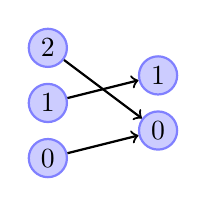
\begin{tikzpicture}[scale=.7,every node/.style={circle,draw=blue!50,fill=blue!20,thick,inner sep=2pt}]
  \node (A) at (0,0) {$0$};
  \node (B) at (0,1) {$1$};
  \node (C) at (0,2) {$2$};
  \node (D) at (2,.5) {$0$};
  \node (E) at (2,1.5) {$1$};
  \draw[->,thick] (A) -- (D);
  \draw[->,thick] (B) -- (E);
  \draw[->,thick] (C) -- (D);
\end{tikzpicture}%
}

\vspace{-5mm}

%\задача
%\выд{Множество всех отображений} из $A$ в $B$ обозначается $B^A$. \hfil \break
%Пусть $\#A=m$, $\#B=n$. Найдите $\#B^A$.
%\кзадача




%\задача
%Пусть $f\colon X\to Y$, $A_1, A_2\subset X$, $B_1, B_2\subset Y$.
%Всегда ли верно, что
%\vspace{-9pt}
%\begin{tabbing}
%\пункт $f(X)=Y$; \hspace{45mm} \=
%\пункт $f^{-1}(Y)=X$;\\
%\пункт $f(A_1\cup A_2)=f(A_1)\cup f(A_2)$; \>
%\пункт $f(A_1\cap A_2)=f(A_1)\cap f(A_2)$; \\
%\пункт $f^{-1}(B_1\cup B_2)=f^{-1}(B_1)\cup f^{-1}(B_2)$; \>
%\пункт $f^{-1}(B_1\cap B_2)=f^{-1}(B_1)\cap f^{-1}(B_2)$; \\
%\пункт если $f(A_1)\subset f(A_2)$, то $A_1\subset A_2$;  \>
%\пункт если $f^{-1}(B_1)\subset f^{-1}(B_2)$, то
%$B_1\subset B_2$.
%\end{tabbing}
%\кзадача

%\vspace{-11pt}



\опр
Отображение $f\colon X\to Y$ называется
\выд{взаимно однозначным} или \\\выд биекцией, если для каждого $y\in Y$ найдётся ровно
один $x\in X$, такой что $f(x)=y$.
\копр

\задача
Какие из отображений задачи \ref{otobraz} взаимно однозначны?
\кзадача



\опр
  Отображение $f$, не \лк склеивающее\пк элементы (то есть $f(x)=f(y)$ только если $x=y$) называется \выд вложением или \выд инъекцией ($A\stackrel{f}{\hookrightarrow}B$). Отображение $f\colon A\to B$, \лк покрывающее\пк все элементы $B$ (то есть $f(A)=B$) называется \выд наложением или \выд сюрьекцией ($A\stackrel{f}{\twoheadrightarrow}B$).
\копр

\задача
Пусть $A$ и $B$~--- конечные множества. Определите в терминах отображений: в множестве~$A$
\пункт меньше;
\пункт больше элементов, чем в множестве $B$;
\пункт столько же элементов, что и в $B$.
\кзадача


\задача
Каких треугольников с целыми сторонами больше:
\сНовойСтроки
\пункт
тех, периметр которых равен
2002, или тех, периметр которых равен 2005?
\пункт
тех, периметр которых равен
2003, или тех, периметр которых равен 2006?
\кзадача


\опр
\выд{Композицией отображений\/} $f\colon X\to Y$ и $g\colon Y\to Z$
называется отображение, сопоставляющее элементу $x$ множества $X$
элемент $g(f(x))$ множества $Z$. Обозначение:~$g\circ f$.
\копр

\задача
Докажите, что для произвольных отображений $f\colon X\to Y$,
$g\colon Y\to Z$ и $h\colon Z\to W$ выполняется
равенство $h\circ(g\circ f)=(h\circ g)\circ f$.
\кзадача


\задача
Пусть $f\colon X\to Y$, $g\colon Y\to Z$. Верно ли, что если $f$ и $g$
взаимно однозначны, то и $g\circ f$ взаимно однозначно?
\кзадача

\задача
Пусть $f\colon X \to Y$ --- взаимно однозначное отображение.
Докажите, что существует и единственно такое отображение $g\colon Y \to X$,
что $g(f(x)) = x$ при любом $x\in X$ и $f(g(y)) = y$ при любом $y\in Y$.
Его называют \выд{обратным к $f$}. Обозначение:~$f^{-1}$.
\кзадача

\задача
Найдите обратные к тем отображениям задачи \ref{otobraz}, которые взаимно однозначны.
\кзадача


\задача
  Докажите, что отображение, обратное к биекции, само есть биекция.
\кзадача



% Композиции

\задача Докажите, что между следующими множествами точек
на прямой есть взаимно однозначное отображение:
\вСтрочку
\пункт любые два отрезка;
\пункт любые два интервала.
\кзадача



\задача
Найдите $g\circ f$, если
\сНовойСтроки
\пункт
$f$ и $g$~--- повороты плоскости относительно одной и той же точки
$O$ на углы $\alpha$ и $\beta$ соответственно.
\пункт
$f$ и $g$~--- симметрии плоскости относительно двух параллельных
прямых $l_1$ и $l_2$ соответственно. %, если $l_1$ и $l_2$ параллельны?
\пункт
$f$ и $g$~--- симметрии плоскости относительно двух непараллельных прямых
$l_1$ и $l_2$ соответственно.
%Рассмотрите все случаи.
\кзадача

%\задача
%Пусть $A$~--- произвольное множество, а в множестве $B$ всего два элемента. Установите взаимно однозначное соответствие между множествами $B^A$ и $2^A$.
%\кзадача

%\задача
%Решите задачу 8в) из листка \No 4 (Комбинаторика).
%\кзадача



%%\СделатьКондуит{6mm}{6.6mm}

%\GenXMLW

\ЛичныйКондуит{0mm}{6mm}\vspace*{-4mm}


\end{document}


















\задача
Некоторое число делится на $2$, но не делится на $4$. Докажите, что
количество ч\"етных делителей этого числа равно количеству
его неч\"етных делителей.
\кзадача

\задача
Каких треугольников с целыми сторонами больше:
\сНовойСтроки
\пункт
тех, периметр которых равен
2002, или тех, периметр которых равен 2005?
\пункт
тех, периметр которых равен
2003, или тех, периметр которых равен 2006?
\кзадача


\задача
Даны три множества: $\N$, множество четных натуральных
чисел и множество натуральных чисел без числа 3.
Про каждые два из этих множеств выясните, существует ли
взаимно однозначное отображение из первого во второе.
%\сНовойСтроки
%\пункт множество натуральных чисел;
%\пункт множество чётных натуральных чисел;
%\пункт множество натуральных чисел без числа 3.
\кзадача

\задача Докажите, что между следующими множествами точек
на прямой есть взаимно однозначное отображение:
\вСтрочку
\пункт любые два отрезка;
\пункт любые два интервала.
\кзадача



\задача
Пусть $f\colon X\to Y$, $A_1, A_2\subset X$, $B_1, B_2\subset Y$.
Всегда ли верно, что
\vspace{-9pt}
\begin{tabbing}
\пункт $f(X)=Y$; \hspace{45mm} \=
\пункт $f^{-1}(Y)=X$;\\
\пункт $f(A_1\cup A_2)=f(A_1)\cup f(A_2)$; \>
\пункт $f(A_1\cap A_2)=f(A_1)\cap f(A_2)$; \\
\пункт $f^{-1}(B_1\cup B_2)=f^{-1}(B_1)\cup f^{-1}(B_2)$; \>
\пункт $f^{-1}(B_1\cap B_2)=f^{-1}(B_1)\cap f^{-1}(B_2)$; \\
\пункт если $f(A_1)\subset f(A_2)$, то $A_1\subset A_2$;  \>
\пункт если $f^{-1}(B_1)\subset f^{-1}(B_2)$, то
$B_1\subset B_2$.
\end{tabbing}
\кзадача

\vspace{-11pt}

